% Options for packages loaded elsewhere
\PassOptionsToPackage{unicode}{hyperref}
\PassOptionsToPackage{hyphens}{url}
%
\documentclass[
]{article}
\usepackage{lmodern}
\usepackage{amssymb,amsmath}
\usepackage{ifxetex,ifluatex}
\ifnum 0\ifxetex 1\fi\ifluatex 1\fi=0 % if pdftex
  \usepackage[T1]{fontenc}
  \usepackage[utf8]{inputenc}
  \usepackage{textcomp} % provide euro and other symbols
\else % if luatex or xetex
  \usepackage{unicode-math}
  \defaultfontfeatures{Scale=MatchLowercase}
  \defaultfontfeatures[\rmfamily]{Ligatures=TeX,Scale=1}
\fi
% Use upquote if available, for straight quotes in verbatim environments
\IfFileExists{upquote.sty}{\usepackage{upquote}}{}
\IfFileExists{microtype.sty}{% use microtype if available
  \usepackage[]{microtype}
  \UseMicrotypeSet[protrusion]{basicmath} % disable protrusion for tt fonts
}{}
\makeatletter
\@ifundefined{KOMAClassName}{% if non-KOMA class
  \IfFileExists{parskip.sty}{%
    \usepackage{parskip}
  }{% else
    \setlength{\parindent}{0pt}
    \setlength{\parskip}{6pt plus 2pt minus 1pt}}
}{% if KOMA class
  \KOMAoptions{parskip=half}}
\makeatother
\usepackage{xcolor}
\IfFileExists{xurl.sty}{\usepackage{xurl}}{} % add URL line breaks if available
\IfFileExists{bookmark.sty}{\usepackage{bookmark}}{\usepackage{hyperref}}
\hypersetup{
  pdftitle={PSA: Three-strategy decision tree in R - HVE},
  pdfauthor={The DARTH workgroup},
  hidelinks,
  pdfcreator={LaTeX via pandoc}}
\urlstyle{same} % disable monospaced font for URLs
\usepackage[margin=1in]{geometry}
\usepackage{color}
\usepackage{fancyvrb}
\newcommand{\VerbBar}{|}
\newcommand{\VERB}{\Verb[commandchars=\\\{\}]}
\DefineVerbatimEnvironment{Highlighting}{Verbatim}{commandchars=\\\{\}}
% Add ',fontsize=\small' for more characters per line
\usepackage{framed}
\definecolor{shadecolor}{RGB}{248,248,248}
\newenvironment{Shaded}{\begin{snugshade}}{\end{snugshade}}
\newcommand{\AlertTok}[1]{\textcolor[rgb]{0.94,0.16,0.16}{#1}}
\newcommand{\AnnotationTok}[1]{\textcolor[rgb]{0.56,0.35,0.01}{\textbf{\textit{#1}}}}
\newcommand{\AttributeTok}[1]{\textcolor[rgb]{0.77,0.63,0.00}{#1}}
\newcommand{\BaseNTok}[1]{\textcolor[rgb]{0.00,0.00,0.81}{#1}}
\newcommand{\BuiltInTok}[1]{#1}
\newcommand{\CharTok}[1]{\textcolor[rgb]{0.31,0.60,0.02}{#1}}
\newcommand{\CommentTok}[1]{\textcolor[rgb]{0.56,0.35,0.01}{\textit{#1}}}
\newcommand{\CommentVarTok}[1]{\textcolor[rgb]{0.56,0.35,0.01}{\textbf{\textit{#1}}}}
\newcommand{\ConstantTok}[1]{\textcolor[rgb]{0.00,0.00,0.00}{#1}}
\newcommand{\ControlFlowTok}[1]{\textcolor[rgb]{0.13,0.29,0.53}{\textbf{#1}}}
\newcommand{\DataTypeTok}[1]{\textcolor[rgb]{0.13,0.29,0.53}{#1}}
\newcommand{\DecValTok}[1]{\textcolor[rgb]{0.00,0.00,0.81}{#1}}
\newcommand{\DocumentationTok}[1]{\textcolor[rgb]{0.56,0.35,0.01}{\textbf{\textit{#1}}}}
\newcommand{\ErrorTok}[1]{\textcolor[rgb]{0.64,0.00,0.00}{\textbf{#1}}}
\newcommand{\ExtensionTok}[1]{#1}
\newcommand{\FloatTok}[1]{\textcolor[rgb]{0.00,0.00,0.81}{#1}}
\newcommand{\FunctionTok}[1]{\textcolor[rgb]{0.00,0.00,0.00}{#1}}
\newcommand{\ImportTok}[1]{#1}
\newcommand{\InformationTok}[1]{\textcolor[rgb]{0.56,0.35,0.01}{\textbf{\textit{#1}}}}
\newcommand{\KeywordTok}[1]{\textcolor[rgb]{0.13,0.29,0.53}{\textbf{#1}}}
\newcommand{\NormalTok}[1]{#1}
\newcommand{\OperatorTok}[1]{\textcolor[rgb]{0.81,0.36,0.00}{\textbf{#1}}}
\newcommand{\OtherTok}[1]{\textcolor[rgb]{0.56,0.35,0.01}{#1}}
\newcommand{\PreprocessorTok}[1]{\textcolor[rgb]{0.56,0.35,0.01}{\textit{#1}}}
\newcommand{\RegionMarkerTok}[1]{#1}
\newcommand{\SpecialCharTok}[1]{\textcolor[rgb]{0.00,0.00,0.00}{#1}}
\newcommand{\SpecialStringTok}[1]{\textcolor[rgb]{0.31,0.60,0.02}{#1}}
\newcommand{\StringTok}[1]{\textcolor[rgb]{0.31,0.60,0.02}{#1}}
\newcommand{\VariableTok}[1]{\textcolor[rgb]{0.00,0.00,0.00}{#1}}
\newcommand{\VerbatimStringTok}[1]{\textcolor[rgb]{0.31,0.60,0.02}{#1}}
\newcommand{\WarningTok}[1]{\textcolor[rgb]{0.56,0.35,0.01}{\textbf{\textit{#1}}}}
\usepackage{graphicx,grffile}
\makeatletter
\def\maxwidth{\ifdim\Gin@nat@width>\linewidth\linewidth\else\Gin@nat@width\fi}
\def\maxheight{\ifdim\Gin@nat@height>\textheight\textheight\else\Gin@nat@height\fi}
\makeatother
% Scale images if necessary, so that they will not overflow the page
% margins by default, and it is still possible to overwrite the defaults
% using explicit options in \includegraphics[width, height, ...]{}
\setkeys{Gin}{width=\maxwidth,height=\maxheight,keepaspectratio}
% Set default figure placement to htbp
\makeatletter
\def\fps@figure{htbp}
\makeatother
\setlength{\emergencystretch}{3em} % prevent overfull lines
\providecommand{\tightlist}{%
  \setlength{\itemsep}{0pt}\setlength{\parskip}{0pt}}
\setcounter{secnumdepth}{-\maxdimen} % remove section numbering

\title{PSA: Three-strategy decision tree in R - HVE}
\author{The DARTH workgroup}
\date{}

\begin{document}
\maketitle

Developed by the Decision Analysis in R for Technologies in Health
(DARTH) workgroup:

Fernando Alarid-Escudero, PhD (1)

Eva A. Enns, MS, PhD (2)

M.G. Myriam Hunink, MD, PhD (3,4)

Hawre J. Jalal, MD, PhD (5)

Eline M. Krijkamp, MSc (3)

Petros Pechlivanoglou, PhD (6,7)

Alan Yang, MSc (7)

In collaboration of:

\begin{enumerate}
\def\labelenumi{\arabic{enumi}.}
\tightlist
\item
  Division of Public Administration, Center for Research and Teaching in
  Economics (CIDE), Aguascalientes, Mexico
\item
  University of Minnesota School of Public Health, Minneapolis, MN, USA
\item
  Erasmus MC, Rotterdam, The Netherlands
\item
  Harvard T.H. Chan School of Public Health, Boston, USA
\item
  University of Pittsburgh Graduate School of Public Health, Pittsburgh,
  PA, USA
\item
  University of Toronto, Toronto ON, Canada
\item
  The Hospital for Sick Children, Toronto ON, Canada
\end{enumerate}

Please cite our publications when using this code:

\begin{itemize}
\item
  Jalal H, Pechlivanoglou P, Krijkamp E, Alarid-Escudero F, Enns E,
  Hunink MG. An Overview of R in Health Decision Sciences. Med Decis
  Making. 2017; 37(3): 735-746.
  \url{https://journals.sagepub.com/doi/abs/10.1177/0272989X16686559}
\item
  Krijkamp EM, Alarid-Escudero F, Enns EA, Jalal HJ, Hunink MGM,
  Pechlivanoglou P. Microsimulation modeling for health decision
  sciences using R: A tutorial. Med Decis Making. 2018;38(3):400--22.
  \url{https://journals.sagepub.com/doi/abs/10.1177/0272989X18754513}
\item
  Krijkamp EM, Alarid-Escudero F, Enns E, Pechlivanoglou P, Hunink MM,
  Jalal H. A Multidimensional Array Representation of State-Transition
  Model Dynamics. Med Decis Making. 2020 Online first.
  \url{https://doi.org/10.1177/0272989X19893973}
\item
  Alarid-Escudero, F., Krijkamp, E. M., Enns, E. A., Hunink, M. G. M.,
  Pechlivanoglou, P., \& Jalal, H. (2020). Cohort state-transition
  models in R: From conceptualization to implementation.
  arXiv:2001.07824v1, 1--31. \url{http://arxiv.org/abs/2001.07824}
\item
  Alarid-Escudero, F., Enns, E. A., Kuntz, K. M., Michaud, T. L., \&
  Jalal, H. (2019). ``Time Traveling Is Just Too Dangerous'' But Some
  Methods Are Worth Revisiting: The Advantages of Expected Loss Curves
  Over Cost-Effectiveness Acceptability Curves and Frontier. Value in
  Health, 22(5), 611--618.
  \url{https://doi.org/10.1016/j.jval.2019.02.008}
\end{itemize}

Copyright 2017, THE HOSPITAL FOR SICK CHILDREN AND THE COLLABORATING
INSTITUTIONS. All rights reserved in Canada, the United States and
worldwide. Copyright, trademarks, trade names and any and all associated
intellectual property are exclusively owned by THE HOSPITAL FOR Sick
CHILDREN and the collaborating institutions. These materials may be
used, reproduced, modified, distributed and adapted with proper
attribution.

\newpage

\begin{Shaded}
\begin{Highlighting}[]
\KeywordTok{rm}\NormalTok{(}\DataTypeTok{list =} \KeywordTok{ls}\NormalTok{())      }\CommentTok{# clear memory (removes all the variables from the workspace)}
\end{Highlighting}
\end{Shaded}

\hypertarget{load-packages}{%
\section{01 Load packages}\label{load-packages}}

\begin{Shaded}
\begin{Highlighting}[]
\ControlFlowTok{if}\NormalTok{ (}\OperatorTok{!}\KeywordTok{require}\NormalTok{(}\StringTok{'pacman'}\NormalTok{)) \{}
  \KeywordTok{install.packages}\NormalTok{(}\StringTok{'pacman'}\NormalTok{)}
\NormalTok{\}}
\KeywordTok{library}\NormalTok{(pacman) }\CommentTok{# use this package to conveniently install other packages}
\CommentTok{# load (install if required) packages from CRAN}
\KeywordTok{p_load}\NormalTok{(}\StringTok{"here"}\NormalTok{, }\StringTok{"dplyr"}\NormalTok{, }\StringTok{"devtools"}\NormalTok{, }\StringTok{"scales"}\NormalTok{, }\StringTok{"ellipse"}\NormalTok{, }\StringTok{"ggplot2"}\NormalTok{, }\StringTok{"lazyeval"}\NormalTok{, }
       \StringTok{"igraph"}\NormalTok{, }\StringTok{"truncnorm"}\NormalTok{, }\StringTok{"ggraph"}\NormalTok{, }\StringTok{"reshape2"}\NormalTok{, }\StringTok{"knitr"}\NormalTok{, }\StringTok{"stringr"}\NormalTok{, }\StringTok{"reshape2"}\NormalTok{)                                            }
\CommentTok{# load (install if required) packages from GitHub}
\CommentTok{# install_github("DARTH-git/dampack", force = TRUE) Uncomment if there is a newer version}
\CommentTok{# install_github("DARTH-git/dectree", force = TRUE) Uncomment if there is a newer version}
\CommentTok{# install_github("annaheath/EVSI", force = TRUE) #Uncomment if there is a newer version}
\KeywordTok{p_load_gh}\NormalTok{(}\StringTok{"DARTH-git/dampack"}\NormalTok{, }\StringTok{"DARTH-git/dectree"}\NormalTok{)}
\KeywordTok{p_load_gh}\NormalTok{(}\StringTok{"annaheath/EVSI"}\NormalTok{)}
\end{Highlighting}
\end{Shaded}

\hypertarget{load-functions}{%
\section{02 Load functions}\label{load-functions}}

\begin{Shaded}
\begin{Highlighting}[]
\KeywordTok{source}\NormalTok{(}\StringTok{"Functions.R"}\NormalTok{)}
\end{Highlighting}
\end{Shaded}

\hypertarget{define-parameter-input-values}{%
\section{03 Define parameter input
values}\label{define-parameter-input-values}}

\begin{Shaded}
\begin{Highlighting}[]
\NormalTok{v_names_str <-}\StringTok{ }\KeywordTok{c}\NormalTok{(}\StringTok{"No Tx"}\NormalTok{, }\StringTok{"Tx All"}\NormalTok{, }\StringTok{"Biopsy"}\NormalTok{) }\CommentTok{# names of strategies}
\NormalTok{n_str       <-}\StringTok{ }\KeywordTok{length}\NormalTok{(v_names_str)            }\CommentTok{# number of strategies}
\NormalTok{wtp         <-}\StringTok{ }\DecValTok{100000}                         \CommentTok{# willingness to pay threshold}

\CommentTok{# Probabilities}
\NormalTok{p_HVE         <-}\StringTok{ }\FloatTok{0.52} \CommentTok{# prevalence of HVE}
\NormalTok{p_HVE_comp    <-}\StringTok{ }\FloatTok{0.71} \CommentTok{# complications with untreated HVE}
\NormalTok{p_OVE_comp    <-}\StringTok{ }\FloatTok{0.01} \CommentTok{# complications with untreated OVE}
\NormalTok{p_HVE_comp_tx <-}\StringTok{ }\FloatTok{0.36} \CommentTok{# complications with treated HVE}
\NormalTok{p_OVE_comp_tx <-}\StringTok{ }\FloatTok{0.20} \CommentTok{# complications with treated OVE}
\NormalTok{p_biopsy_comp <-}\StringTok{ }\FloatTok{0.05} \CommentTok{# probability of complications due to biopsy}

\CommentTok{# Costs}
\NormalTok{c_VE      <-}\StringTok{ }\DecValTok{1200}  \CommentTok{# cost of viral encephalitis care without complications}
\NormalTok{c_VE_comp <-}\StringTok{ }\DecValTok{9000}  \CommentTok{# cost of viral encephalitis care with complications}
\NormalTok{c_tx      <-}\StringTok{ }\DecValTok{9500}  \CommentTok{# cost of treatment}
\NormalTok{c_biopsy  <-}\StringTok{ }\DecValTok{25000} \CommentTok{# cost of brain biopsy}

\CommentTok{# QALYs}
\NormalTok{q_VE          <-}\StringTok{ }\DecValTok{20}    \CommentTok{# remaining QALYs for those without VE-related complications}
\NormalTok{q_VE_comp     <-}\StringTok{ }\DecValTok{19}    \CommentTok{# remaining QALYs for those with VE-related complications}
\NormalTok{q_loss_biopsy <-}\StringTok{ }\FloatTok{-0.01} \CommentTok{# one-time QALY loss due to brain biopsy}

\CommentTok{# store the parameters into a list}
\NormalTok{l_params_all <-}\StringTok{ }\KeywordTok{list}\NormalTok{(p_HVE, p_HVE_comp, p_OVE_comp, p_HVE_comp_tx, }
\NormalTok{                     p_OVE_comp_tx, p_biopsy_comp, }
\NormalTok{                     c_VE, c_VE_comp, c_tx, c_biopsy, }
\NormalTok{                     q_VE, q_VE_comp, q_loss_biopsy)}
\CommentTok{# store the names of the parameters into a vector}
\NormalTok{v_names_params <-}\StringTok{ }\KeywordTok{c}\NormalTok{(}\StringTok{'p_HVE'}\NormalTok{, }\StringTok{'p_HVE_comp'}\NormalTok{, }\StringTok{'p_OVE_comp'}\NormalTok{, }\StringTok{'p_HVE_comp_tx'}\NormalTok{, }
                    \StringTok{'p_OVE_comp_tx'}\NormalTok{, }\StringTok{'p_biopsy_comp'}\NormalTok{, }
                    \StringTok{'c_VE'}\NormalTok{, }\StringTok{'c_VE_comp'}\NormalTok{,  }\StringTok{'c_tx'}\NormalTok{, }\StringTok{'c_biopsy'}\NormalTok{, }
                    \StringTok{'q_VE'}\NormalTok{, }\StringTok{'q_VE_comp'}\NormalTok{, }\StringTok{'q_loss_biopsy'}\NormalTok{)}
\KeywordTok{names}\NormalTok{(l_params_all) <-}\StringTok{ }\NormalTok{v_names_params}
\end{Highlighting}
\end{Shaded}

\hypertarget{create-and-run-decision-tree-model}{%
\section{04 Create and run decision tree
model}\label{create-and-run-decision-tree-model}}

\begin{Shaded}
\begin{Highlighting}[]
\NormalTok{decision_tree_HVE_output <-}\StringTok{ }\KeywordTok{with}\NormalTok{(}\KeywordTok{as.list}\NormalTok{(l_params_all), \{}
  
  \CommentTok{# Create vector of weights for each strategy }
  
\NormalTok{  v_w_no_tx  <-}\StringTok{ }\KeywordTok{c}\NormalTok{(  p_HVE  }\OperatorTok{*}\StringTok{    }\NormalTok{p_HVE_comp  ,  }\CommentTok{# HVE, complications}
\NormalTok{                    p_HVE  }\OperatorTok{*}\StringTok{ }\NormalTok{(}\DecValTok{1}\OperatorTok{-}\NormalTok{p_HVE_comp) ,  }\CommentTok{# HVE, no complications}
\NormalTok{                 (}\DecValTok{1}\OperatorTok{-}\NormalTok{p_HVE) }\OperatorTok{*}\StringTok{    }\NormalTok{p_OVE_comp  ,  }\CommentTok{# OVE, complications}
\NormalTok{                 (}\DecValTok{1}\OperatorTok{-}\NormalTok{p_HVE) }\OperatorTok{*}\StringTok{ }\NormalTok{(}\DecValTok{1}\OperatorTok{-}\NormalTok{p_OVE_comp))   }\CommentTok{# OVE, no complications}
  
\NormalTok{  v_w_tx     <-}\StringTok{ }\KeywordTok{c}\NormalTok{(  }\DecValTok{1}\NormalTok{                          ,  }\CommentTok{# On treatment}
\NormalTok{                    p_HVE  }\OperatorTok{*}\StringTok{    }\NormalTok{p_HVE_comp_tx  ,  }\CommentTok{# HVE w/tx, complications}
\NormalTok{                    p_HVE  }\OperatorTok{*}\StringTok{ }\NormalTok{(}\DecValTok{1}\OperatorTok{-}\NormalTok{p_HVE_comp_tx) ,  }\CommentTok{# HVE w/tx, no complications}
\NormalTok{                 (}\DecValTok{1}\OperatorTok{-}\NormalTok{p_HVE) }\OperatorTok{*}\StringTok{    }\NormalTok{p_OVE_comp_tx  ,  }\CommentTok{# OVE w/tx, complications}
\NormalTok{                 (}\DecValTok{1}\OperatorTok{-}\NormalTok{p_HVE) }\OperatorTok{*}\StringTok{ }\NormalTok{(}\DecValTok{1}\OperatorTok{-}\NormalTok{p_OVE_comp_tx))   }\CommentTok{# OVE w/tx, no complications}
  
\NormalTok{  v_w_biopsy <-}\StringTok{ }\KeywordTok{c}\NormalTok{(}\DecValTok{1}\NormalTok{                                     , }\CommentTok{# Undergo biopsy}
\NormalTok{                  p_biopsy_comp                         , }\CommentTok{# biopsy complications}
                 \CommentTok{# no biopsy comp., HVE w/tx,  complications}
\NormalTok{                 (}\DecValTok{1}\OperatorTok{-}\NormalTok{p_biopsy_comp) }\OperatorTok{*}\StringTok{    }\NormalTok{p_HVE  }\OperatorTok{*}\StringTok{    }\NormalTok{p_HVE_comp_tx ,  }
                 \CommentTok{# no biopsy comp., HVE w/tx, no complications}
\NormalTok{                 (}\DecValTok{1}\OperatorTok{-}\NormalTok{p_biopsy_comp) }\OperatorTok{*}\StringTok{    }\NormalTok{p_HVE  }\OperatorTok{*}\StringTok{ }\NormalTok{(}\DecValTok{1}\OperatorTok{-}\NormalTok{p_HVE_comp_tx),  }
                 \CommentTok{# no biopsy comp., OVE, complications}
\NormalTok{                 (}\DecValTok{1}\OperatorTok{-}\NormalTok{p_biopsy_comp) }\OperatorTok{*}\StringTok{ }\NormalTok{(}\DecValTok{1}\OperatorTok{-}\NormalTok{p_HVE) }\OperatorTok{*}\StringTok{    }\NormalTok{p_OVE_comp    ,  }
                 \CommentTok{# no biopsy comp., OVE, no complications}
\NormalTok{                 (}\DecValTok{1}\OperatorTok{-}\NormalTok{p_biopsy_comp) }\OperatorTok{*}\StringTok{ }\NormalTok{(}\DecValTok{1}\OperatorTok{-}\NormalTok{p_HVE) }\OperatorTok{*}\StringTok{ }\NormalTok{(}\DecValTok{1}\OperatorTok{-}\NormalTok{p_OVE_comp))      }
  
  \CommentTok{# Create vector of outcomes (QALYs) for each strategy }
  
\NormalTok{  v_qaly_no_tx  <-}\StringTok{ }\KeywordTok{c}\NormalTok{(q_VE_comp, }\CommentTok{# HVE, complications}
\NormalTok{                     q_VE     , }\CommentTok{# HVE, no complications}
\NormalTok{                     q_VE_comp, }\CommentTok{# OVE, complications}
\NormalTok{                     q_VE)      }\CommentTok{# OVE, no complications}
  
\NormalTok{  v_qaly_tx     <-}\StringTok{ }\KeywordTok{c}\NormalTok{(}\DecValTok{0}\NormalTok{         , }\CommentTok{# treatment does not directly add any QALYs }
\NormalTok{                     q_VE_comp , }\CommentTok{# HVE, complications}
\NormalTok{                     q_VE      , }\CommentTok{# HVE, no complications}
\NormalTok{                     q_VE_comp , }\CommentTok{# OVE, complications}
\NormalTok{                     q_VE)       }\CommentTok{# OVE, no complications}
  
  
\NormalTok{  v_qaly_biopsy <-}\StringTok{ }\KeywordTok{c}\NormalTok{(q_loss_biopsy, }\CommentTok{# loss due to biopsy}
\NormalTok{                     q_VE_comp    , }\CommentTok{# biopsy complications}
\NormalTok{                     q_VE_comp    , }\CommentTok{# no biopsy comp., HVE w/tx, complications }
\NormalTok{                     q_VE         , }\CommentTok{# no biopsy comp., HVE w/tx, no complications}
\NormalTok{                     q_VE_comp    , }\CommentTok{# no biopsy comp., OVE, complications}
\NormalTok{                     q_VE)          }\CommentTok{# no biopsy comp., OVE, no complications}
  
  \CommentTok{# Create vector of costs for each strategy }
  
\NormalTok{  v_cost_no_tx  <-}\StringTok{ }\KeywordTok{c}\NormalTok{(c_VE_comp , }\CommentTok{# HVE, complications}
\NormalTok{                     c_VE      , }\CommentTok{# HVE, no complications}
\NormalTok{                     c_VE_comp , }\CommentTok{# OVE, complications}
\NormalTok{                     c_VE)       }\CommentTok{# OVE, no complications}
  
\NormalTok{  v_cost_tx     <-}\StringTok{ }\KeywordTok{c}\NormalTok{(c_tx      , }\CommentTok{# cost of treatment}
\NormalTok{                     c_VE_comp , }\CommentTok{# HVE, complications}
\NormalTok{                     c_VE      , }\CommentTok{# HVE, no complications}
\NormalTok{                     c_VE_comp , }\CommentTok{# OVE, complications}
\NormalTok{                     c_VE)       }\CommentTok{# OVE, no complications}
  
  
\NormalTok{  v_cost_biopsy <-}\StringTok{ }\KeywordTok{c}\NormalTok{(c_biopsy         , }\CommentTok{# cost of biopsy procedure}
\NormalTok{                     c_VE_comp        , }\CommentTok{# biopsy complications}
\NormalTok{                     c_VE_comp }\OperatorTok{+}\StringTok{ }\NormalTok{c_tx , }\CommentTok{# no biopsy comp., HVE w/tx, complications }
\NormalTok{                     c_VE }\OperatorTok{+}\StringTok{ }\NormalTok{c_tx      , }\CommentTok{# no biopsy comp., HVE w/tx, no complications}
\NormalTok{                     c_VE_comp        , }\CommentTok{# no biopsy comp., OVE, complications}
\NormalTok{                     c_VE)              }\CommentTok{# no biopsy comp., OVE, no complications}
  
  \CommentTok{# Calculate total utilities for each strategy }
\NormalTok{  total_qaly_no_tx  <-}\StringTok{ }\NormalTok{v_w_no_tx  }\OperatorTok\StringTok{ }\NormalTok{v_qaly_no_tx      }
\NormalTok{  total_qaly_tx     <-}\StringTok{ }\NormalTok{v_w_tx     }\OperatorTok\StringTok{ }\NormalTok{v_qaly_tx}
\NormalTok{  total_qaly_biopsy <-}\StringTok{ }\NormalTok{v_w_biopsy }\OperatorTok\StringTok{ }\NormalTok{v_qaly_biopsy}
  
  \CommentTok{# Calculate total costs for each strategy }
\NormalTok{  total_cost_no_tx  <-}\StringTok{ }\NormalTok{v_w_no_tx  }\OperatorTok\StringTok{ }\NormalTok{v_cost_no_tx    }
\NormalTok{  total_cost_tx     <-}\StringTok{ }\NormalTok{v_w_tx     }\OperatorTok\StringTok{ }\NormalTok{v_cost_tx}
\NormalTok{  total_cost_biopsy <-}\StringTok{ }\NormalTok{v_w_biopsy }\OperatorTok\StringTok{ }\NormalTok{v_cost_biopsy}
  
  \CommentTok{# vector of total QALYs}
\NormalTok{  v_total_qaly <-}\StringTok{ }\KeywordTok{c}\NormalTok{(total_qaly_no_tx, total_qaly_tx, total_qaly_biopsy) }
  \CommentTok{# vector of total costs}
\NormalTok{  v_total_cost <-}\StringTok{ }\KeywordTok{c}\NormalTok{(total_cost_no_tx, total_cost_tx, total_cost_biopsy) }
  \CommentTok{# calculate vector of nmb}
\NormalTok{  v_nmb        <-}\StringTok{ }\NormalTok{v_total_qaly }\OperatorTok{*}\StringTok{ }\NormalTok{wtp }\OperatorTok{-}\StringTok{ }\NormalTok{v_total_cost                      }
  
  \CommentTok{# Name outcomes}
  \KeywordTok{names}\NormalTok{(v_total_qaly) <-}\StringTok{ }\NormalTok{v_names_str  }\CommentTok{# names for the elements of the total QALYs vector}
  \KeywordTok{names}\NormalTok{(v_total_cost) <-}\StringTok{ }\NormalTok{v_names_str  }\CommentTok{# names for the elements of the total cost vector}
  \KeywordTok{names}\NormalTok{(v_nmb)        <-}\StringTok{ }\NormalTok{v_names_str  }\CommentTok{# names for the elements of the nmb vector}
  
\NormalTok{  df_output <-}\StringTok{ }\KeywordTok{data.frame}\NormalTok{(}\DataTypeTok{Strategy =}\NormalTok{ v_names_str,}
                          \DataTypeTok{Cost     =}\NormalTok{ v_total_cost,}
                          \DataTypeTok{Effect   =}\NormalTok{ v_total_qaly,}
                          \DataTypeTok{NMB      =}\NormalTok{ v_nmb)}
  \KeywordTok{return}\NormalTok{(df_output)}
\NormalTok{\})}

\CommentTok{# model output}
\NormalTok{decision_tree_HVE_output}
\end{Highlighting}
\end{Shaded}

\begin{verbatim}
##        Strategy     Cost  Effect     NMB
## No Tx     No Tx  4117.20 19.6260 1958483
## Tx All   Tx All 12908.96 19.7168 1958771
## Biopsy   Biopsy 32705.72 19.7576 1943054
\end{verbatim}

\hypertarget{plot-the-decision-tree}{%
\subsection{04.1 Plot the decision tree}\label{plot-the-decision-tree}}

\begin{Shaded}
\begin{Highlighting}[]
\CommentTok{# branches <- read.csv(here('data','decision_tree_HVE_branches.csv'), }
\CommentTok{#                      stringsAsFactors = F, header = T)}
\CommentTok{# tree     <- create_tree(branches)}
\CommentTok{# plot_tree(tree, font.size = 5)}
\end{Highlighting}
\end{Shaded}

\hypertarget{cost-effectiveness-analysis}{%
\subsection{05 Cost-Effectiveness
Analysis}\label{cost-effectiveness-analysis}}

\begin{Shaded}
\begin{Highlighting}[]
\CommentTok{# create the transition probability matrix for NO treatment}
\NormalTok{decision_tree_HVE_cea  <-}\StringTok{ }\KeywordTok{calculate_icers}\NormalTok{(}\DataTypeTok{cost       =}\NormalTok{ decision_tree_HVE_output}\OperatorTok{$}\NormalTok{Cost,}
                                          \DataTypeTok{effect     =}\NormalTok{ decision_tree_HVE_output}\OperatorTok{$}\NormalTok{Effect,}
                                          \DataTypeTok{strategies =}\NormalTok{ decision_tree_HVE_output}\OperatorTok{$}\NormalTok{Strategy)}
\NormalTok{decision_tree_HVE_cea}
\end{Highlighting}
\end{Shaded}

\begin{verbatim}
##   Strategy     Cost  Effect Inc_Cost Inc_Effect      ICER Status
## 1    No Tx  4117.20 19.6260       NA         NA        NA     ND
## 2   Tx All 12908.96 19.7168  8791.76     0.0908  96825.55     ND
## 3   Biopsy 32705.72 19.7576 19796.76     0.0408 485214.71     ND
\end{verbatim}

\hypertarget{plot-frontier-of-decision-tree}{%
\subsection{05.1 Plot frontier of Decision
Tree}\label{plot-frontier-of-decision-tree}}

\begin{Shaded}
\begin{Highlighting}[]
\KeywordTok{plot}\NormalTok{(decision_tree_HVE_cea, }\DataTypeTok{effect_units =} \StringTok{"QALYs"}\NormalTok{)}
\end{Highlighting}
\end{Shaded}

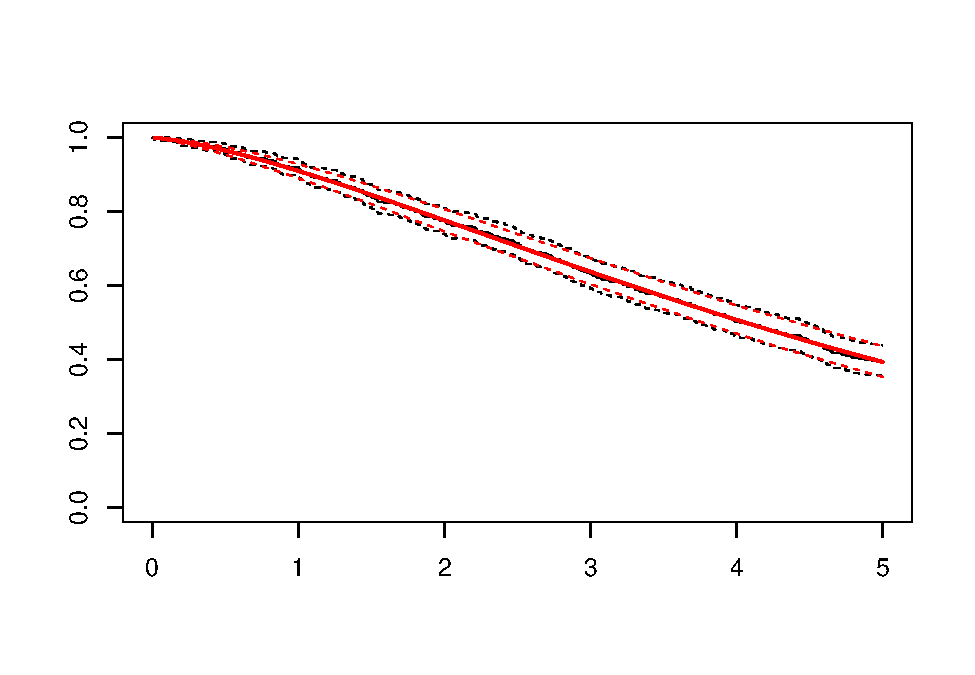
\includegraphics{decision_tree_HVE_PSA_solutions_files/figure-latex/unnamed-chunk-8-1.pdf}

\hypertarget{deterministic-sensitivity-analysis}{%
\section{06 Deterministic Sensitivity
Analysis}\label{deterministic-sensitivity-analysis}}

\hypertarget{list-of-input-parameters}{%
\subsection{06.1 List of input
parameters}\label{list-of-input-parameters}}

\begin{Shaded}
\begin{Highlighting}[]
\NormalTok{l_params_all }
\end{Highlighting}
\end{Shaded}

\begin{verbatim}
## $p_HVE
## [1] 0.52
## 
## $p_HVE_comp
## [1] 0.71
## 
## $p_OVE_comp
## [1] 0.01
## 
## $p_HVE_comp_tx
## [1] 0.36
## 
## $p_OVE_comp_tx
## [1] 0.2
## 
## $p_biopsy_comp
## [1] 0.05
## 
## $c_VE
## [1] 1200
## 
## $c_VE_comp
## [1] 9000
## 
## $c_tx
## [1] 9500
## 
## $c_biopsy
## [1] 25000
## 
## $q_VE
## [1] 20
## 
## $q_VE_comp
## [1] 19
## 
## $q_loss_biopsy
## [1] -0.01
\end{verbatim}

\hypertarget{load-decision-tree-model-function}{%
\subsection{06.2 Load decision tree model
function}\label{load-decision-tree-model-function}}

\begin{Shaded}
\begin{Highlighting}[]
\CommentTok{#### We wrapped the decision tree in a function which we called calculate_ce_out }
\CommentTok{# This function is stored in "Functions_decision_tree_HVE.R" and needes the list of parameters}
\KeywordTok{source}\NormalTok{(}\StringTok{"Functions_decision_tree_HVE.R"}\NormalTok{)}
\CommentTok{# Test function to see if it gives the CE results}
\KeywordTok{calculate_ce_out}\NormalTok{(l_params_all)}
\end{Highlighting}
\end{Shaded}

\begin{verbatim}
##        Strategy     Cost  Effect     NMB
## No Tx     No Tx  4117.20 19.6260 1958483
## Tx All   Tx All 12908.96 19.7168 1958771
## Biopsy   Biopsy 32705.72 19.7576 1943054
\end{verbatim}

\hypertarget{one-way-sensitivity-analysis-owsa}{%
\subsection{06.3 One-way sensitivity analysis
(OWSA)}\label{one-way-sensitivity-analysis-owsa}}

\begin{Shaded}
\begin{Highlighting}[]
\KeywordTok{options}\NormalTok{(}\DataTypeTok{scipen =} \DecValTok{999}\NormalTok{) }\CommentTok{# disabling scientific notation in R}
\CommentTok{# dataframe containing all parameters, their basecase values, and the min and }
\CommentTok{# max values of the parameters of interest }
\NormalTok{df_params_owsa <-}\StringTok{ }\KeywordTok{data.frame}\NormalTok{(}\DataTypeTok{pars =} \KeywordTok{c}\NormalTok{(}\StringTok{"p_HVE"}\NormalTok{, }\StringTok{"p_biopsy_comp"}\NormalTok{, }\StringTok{"c_tx"}\NormalTok{, }\StringTok{"c_biopsy"}\NormalTok{),}
                             \DataTypeTok{min  =} \KeywordTok{c}\NormalTok{(}\FloatTok{0.01}\NormalTok{, }\FloatTok{0.01}\NormalTok{,  }\DecValTok{1000}\NormalTok{, }\DecValTok{5000}\NormalTok{),  }\CommentTok{# min parameter values}
                             \DataTypeTok{max  =} \KeywordTok{c}\NormalTok{(}\FloatTok{0.99}\NormalTok{, }\FloatTok{0.50}\NormalTok{, }\DecValTok{15000}\NormalTok{, }\DecValTok{40000}\NormalTok{)  }\CommentTok{# max parameter values}
\NormalTok{                             )}

\NormalTok{owsa_nmb <-}\StringTok{ }\KeywordTok{run_owsa_det}\NormalTok{(}\DataTypeTok{params_range =}\NormalTok{ df_params_owsa,  }\CommentTok{# dataframe with parameters for owsa}
                         \DataTypeTok{params_basecase =}\NormalTok{ l_params_all, }\CommentTok{# list with all parameters}
                         \DataTypeTok{nsamp      =} \DecValTok{100}\NormalTok{,               }\CommentTok{# number of parameter values}
                         \DataTypeTok{FUN        =}\NormalTok{ calculate_ce_out,  }\CommentTok{# function to compute outputs}
                         \DataTypeTok{outcomes   =} \KeywordTok{c}\NormalTok{(}\StringTok{"NMB"}\NormalTok{),          }\CommentTok{# output to do the OWSA on}
                         \DataTypeTok{strategies =}\NormalTok{ v_names_str,       }\CommentTok{# names of the strategies}
                         \DataTypeTok{n_wtp      =} \DecValTok{450000}\NormalTok{)            }\CommentTok{# extra argument to pass to FUN}
\end{Highlighting}
\end{Shaded}

\hypertarget{plot-owsa}{%
\subsection{06.3.1 Plot OWSA}\label{plot-owsa}}

\begin{Shaded}
\begin{Highlighting}[]
\KeywordTok{plot}\NormalTok{(owsa_nmb, }\DataTypeTok{txtsize =} \DecValTok{16}\NormalTok{, }\DataTypeTok{n_x_ticks =} \DecValTok{5}\NormalTok{, }\DataTypeTok{n_y_ticks =} \DecValTok{3}\NormalTok{,}
     \DataTypeTok{facet_scales =} \StringTok{"free"}\NormalTok{) }\OperatorTok{+}
\StringTok{     }\KeywordTok{theme}\NormalTok{(}\DataTypeTok{legend.position =} \StringTok{"bottom"}\NormalTok{, }
           \DataTypeTok{axis.text.x =} \KeywordTok{element_text}\NormalTok{(}\DataTypeTok{angle =} \DecValTok{45}\NormalTok{, }\DataTypeTok{vjust =} \FloatTok{0.5}\NormalTok{))}
\end{Highlighting}
\end{Shaded}

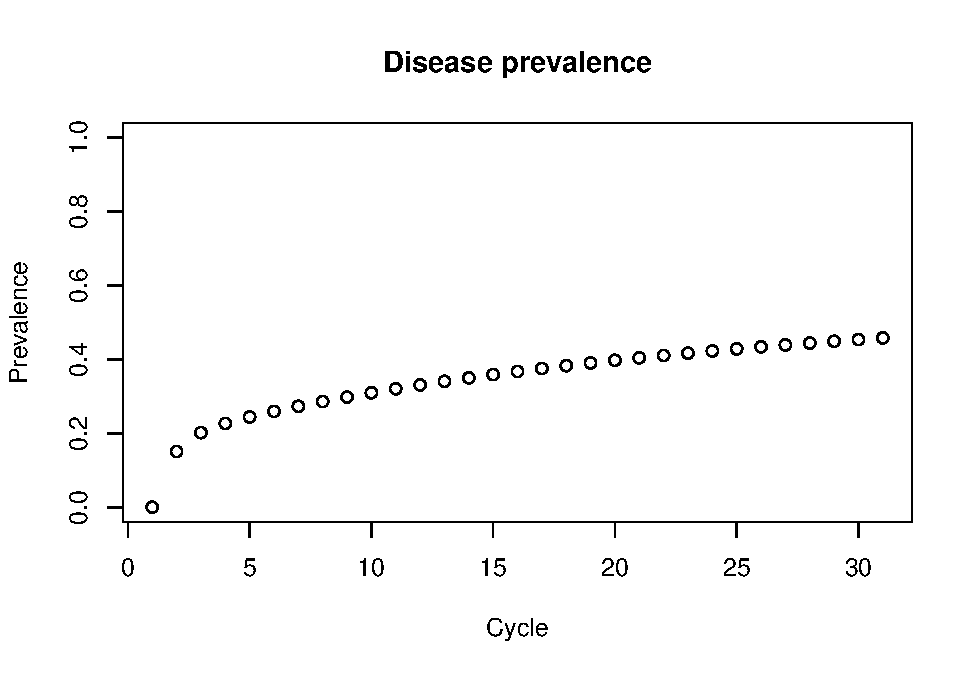
\includegraphics{decision_tree_HVE_PSA_solutions_files/figure-latex/unnamed-chunk-12-1.pdf}

\hypertarget{optimal-strategy-with-owsa}{%
\subsection{06.3.2 Optimal strategy with
OWSA}\label{optimal-strategy-with-owsa}}

\begin{Shaded}
\begin{Highlighting}[]
\KeywordTok{owsa_opt_strat}\NormalTok{(}\DataTypeTok{owsa =}\NormalTok{ owsa_nmb)}
\end{Highlighting}
\end{Shaded}

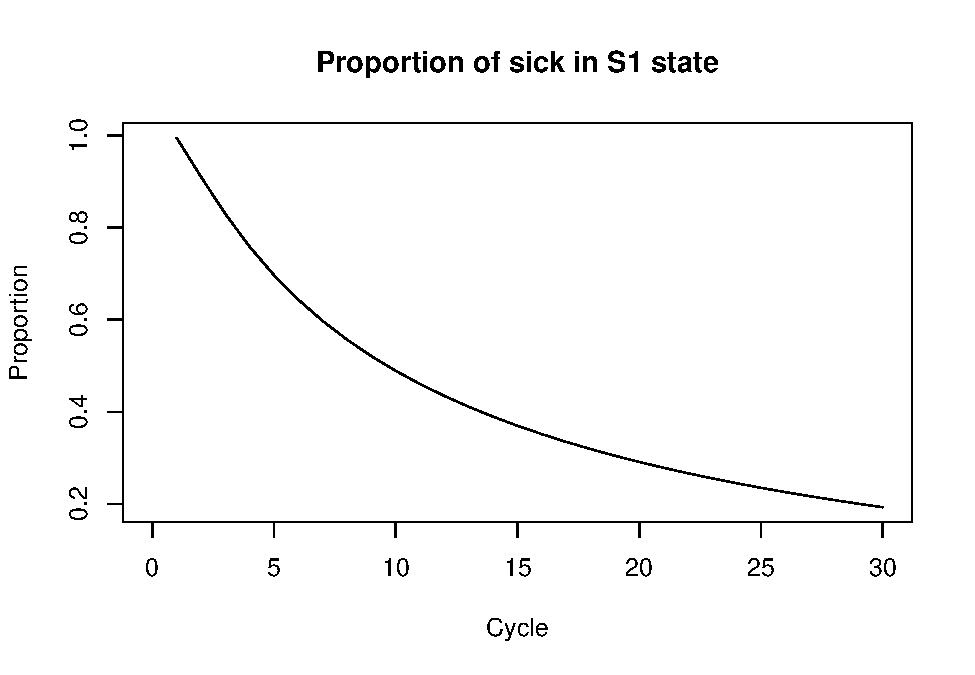
\includegraphics{decision_tree_HVE_PSA_solutions_files/figure-latex/unnamed-chunk-13-1.pdf}

\hypertarget{tornado-plot}{%
\subsection{06.3.3 Tornado plot}\label{tornado-plot}}

\begin{Shaded}
\begin{Highlighting}[]
\KeywordTok{owsa_tornado}\NormalTok{(}\DataTypeTok{owsa =}\NormalTok{ owsa_nmb) }\OperatorTok{+}
\StringTok{  }\KeywordTok{theme}\NormalTok{(}\DataTypeTok{axis.text.x =} \KeywordTok{element_text}\NormalTok{(}\DataTypeTok{angle =} \DecValTok{45}\NormalTok{, }\DataTypeTok{vjust =} \FloatTok{0.5}\NormalTok{))}
\end{Highlighting}
\end{Shaded}

\includegraphics{decision_tree_HVE_PSA_solutions_files/figure-latex/unnamed-chunk-14-1.pdf}

\hypertarget{two-way-sensitivity-analysis-twsa}{%
\subsection{06.4 Two-way sensitivity analysis
(TWSA)}\label{two-way-sensitivity-analysis-twsa}}

\begin{Shaded}
\begin{Highlighting}[]
\CommentTok{# dataframe containing all parameters, their basecase values, and the min and }
\CommentTok{# max values of the parameters of interest}
\NormalTok{df_params_twsa <-}\StringTok{ }\KeywordTok{data.frame}\NormalTok{(}\DataTypeTok{pars =} \KeywordTok{c}\NormalTok{(}\StringTok{"p_HVE"}\NormalTok{, }\StringTok{"c_biopsy"}\NormalTok{),}
                              \DataTypeTok{min  =} \KeywordTok{c}\NormalTok{(}\FloatTok{0.01}\NormalTok{, }\DecValTok{2000}\NormalTok{), }\CommentTok{# min parameter values}
                              \DataTypeTok{max  =} \KeywordTok{c}\NormalTok{(}\FloatTok{0.99}\NormalTok{, }\DecValTok{40000}\NormalTok{) }\CommentTok{# max parameter values}
\NormalTok{                              )}

\NormalTok{twsa_nmb <-}\StringTok{ }\KeywordTok{run_twsa_det}\NormalTok{(}\DataTypeTok{params_range =}\NormalTok{ df_params_twsa, }\CommentTok{# dataframe with parameters for twsa}
                         \DataTypeTok{params_basecase =}\NormalTok{ l_params_all,}\CommentTok{# list with all parameters}
                         \DataTypeTok{nsamp      =} \DecValTok{40}\NormalTok{,               }\CommentTok{# number of parameter values}
                         \DataTypeTok{FUN        =}\NormalTok{ calculate_ce_out, }\CommentTok{# function to compute outputs}
                         \DataTypeTok{outcomes   =} \KeywordTok{c}\NormalTok{(}\StringTok{"NMB"}\NormalTok{),         }\CommentTok{# output to do the twsa on}
                         \DataTypeTok{strategies =}\NormalTok{ v_names_str,      }\CommentTok{# names of the strategies}
                         \DataTypeTok{n_wtp      =} \DecValTok{200000}\NormalTok{)           }\CommentTok{# extra argument to pass to FUN}
\end{Highlighting}
\end{Shaded}

\hypertarget{plot-twsa}{%
\subsection{06.4.1 Plot TWSA}\label{plot-twsa}}

\begin{Shaded}
\begin{Highlighting}[]
\KeywordTok{plot}\NormalTok{(twsa_nmb) }\OperatorTok{+}\StringTok{ }
\StringTok{  }\KeywordTok{ggtitle}\NormalTok{(}\DataTypeTok{label =} \StringTok{"Two-way sensitivity analysis"}\NormalTok{, }
          \DataTypeTok{subtitle =} \StringTok{"Net monetary benefit"}\NormalTok{) }\OperatorTok{+}
\StringTok{          }\KeywordTok{theme}\NormalTok{(}\DataTypeTok{legend.position =} \StringTok{"bottom"}\NormalTok{)}
\end{Highlighting}
\end{Shaded}

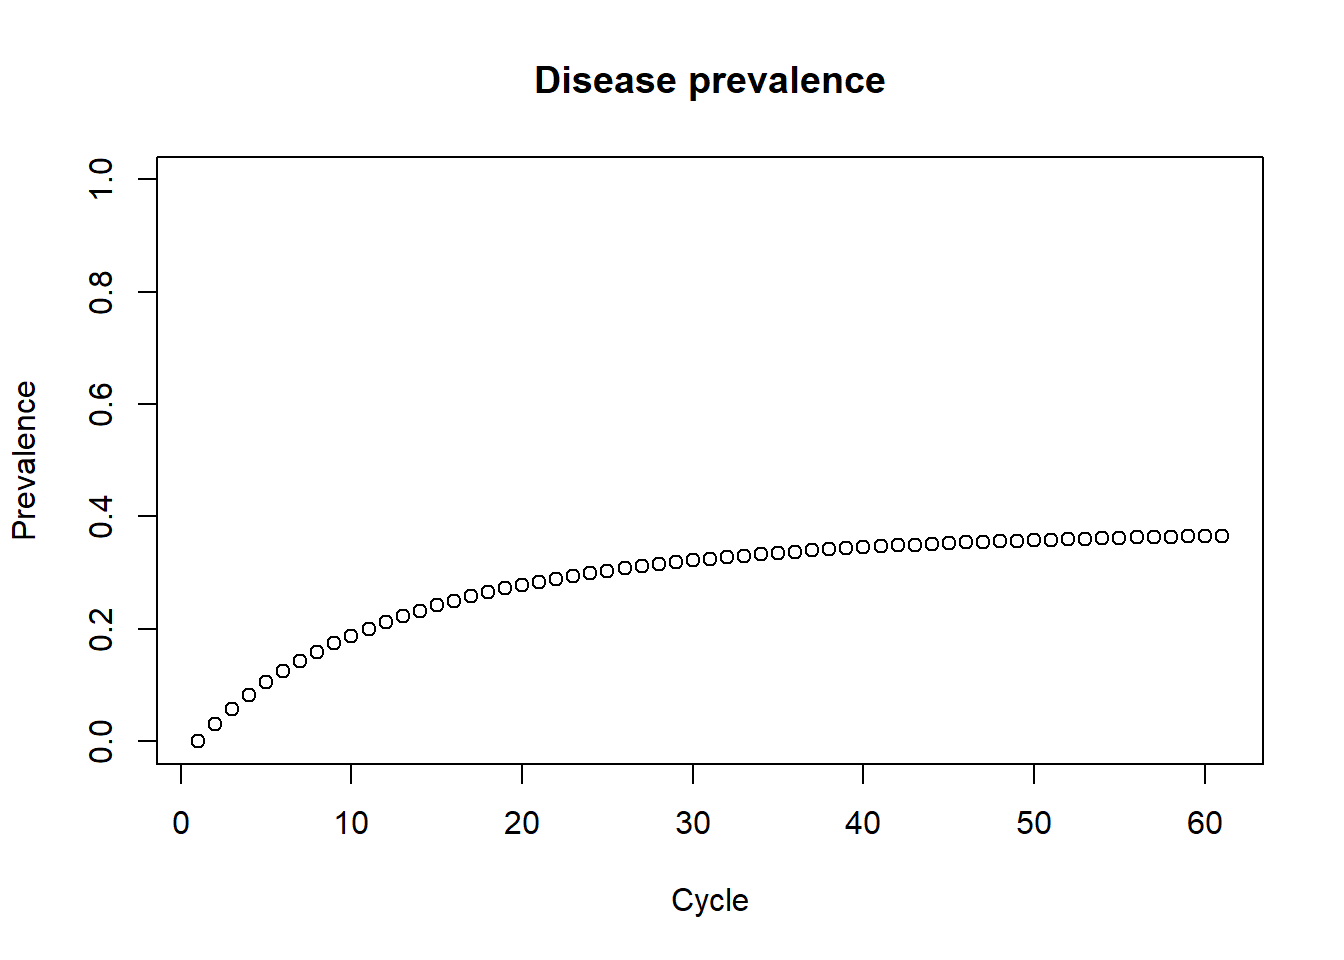
\includegraphics{decision_tree_HVE_PSA_solutions_files/figure-latex/unnamed-chunk-16-1.pdf}

\hypertarget{probabilistic-sensitivity-analysis-psa}{%
\section{07 Probabilistic Sensitivity Analysis
(PSA)}\label{probabilistic-sensitivity-analysis-psa}}

\begin{Shaded}
\begin{Highlighting}[]
\CommentTok{# Function to generate PSA input dataset}
\NormalTok{generate_psa_params <-}\StringTok{ }\ControlFlowTok{function}\NormalTok{(}\DataTypeTok{n_sim =} \DecValTok{1000}\NormalTok{, }\DataTypeTok{seed =} \DecValTok{071518}\NormalTok{)\{}
  \KeywordTok{set.seed}\NormalTok{(seed)}
  \CommentTok{# Dataframe of input parameters}
\NormalTok{  df_psa_params   <-}\StringTok{ }\KeywordTok{data.frame}\NormalTok{(}
    
    \CommentTok{# Transition probabilities (per cycle)}
    \DataTypeTok{p_HVE         =} \KeywordTok{rbeta}\NormalTok{(n_sim, }\DecValTok{52}\NormalTok{, }\DecValTok{48}\NormalTok{), }\CommentTok{# prevalence of HVE}
    \DataTypeTok{p_HVE_comp    =} \KeywordTok{rbeta}\NormalTok{(n_sim, }\DecValTok{71}\NormalTok{, }\DecValTok{29}\NormalTok{), }\CommentTok{# complications with untreated HVE}
    \DataTypeTok{p_OVE_comp    =} \KeywordTok{rbeta}\NormalTok{(n_sim,  }\DecValTok{1}\NormalTok{, }\DecValTok{99}\NormalTok{), }\CommentTok{# complications with untreated OVE}
    \DataTypeTok{p_HVE_comp_tx =} \KeywordTok{rbeta}\NormalTok{(n_sim, }\DecValTok{36}\NormalTok{, }\DecValTok{64}\NormalTok{), }\CommentTok{# complications with treated HVE}
    \DataTypeTok{p_OVE_comp_tx =} \KeywordTok{rbeta}\NormalTok{(n_sim, }\DecValTok{20}\NormalTok{, }\DecValTok{80}\NormalTok{), }\CommentTok{# complications with treated OVE}
    \DataTypeTok{p_biopsy_comp =} \KeywordTok{rbeta}\NormalTok{(n_sim,  }\DecValTok{1}\NormalTok{, }\DecValTok{19}\NormalTok{), }\CommentTok{# probability of complications due to biopsy}
    
    \CommentTok{# Costs}
    \DataTypeTok{c_VE      =} \KeywordTok{rgamma}\NormalTok{(n_sim, }\DataTypeTok{shape =} \FloatTok{36.0}\NormalTok{, }\DataTypeTok{scale =} \FloatTok{33.33}\NormalTok{), }\CommentTok{# cost of remaining one cycle in state H}
    \DataTypeTok{c_VE_comp =} \KeywordTok{rgamma}\NormalTok{(n_sim, }\DataTypeTok{shape =} \FloatTok{81.0}\NormalTok{, }\DataTypeTok{scale =} \FloatTok{111.1}\NormalTok{), }\CommentTok{# cost of remaining one cycle in state S1}
    \DataTypeTok{c_tx      =} \KeywordTok{rgamma}\NormalTok{(n_sim, }\DataTypeTok{shape =} \FloatTok{74.6}\NormalTok{, }\DataTypeTok{scale =} \FloatTok{127.4}\NormalTok{), }\CommentTok{# cost of remaining one cycle in state S2}
    \DataTypeTok{c_biopsy  =} \KeywordTok{rgamma}\NormalTok{(n_sim, }\DataTypeTok{shape =} \FloatTok{25.0}\NormalTok{, }\DataTypeTok{scale =} \DecValTok{1000}\NormalTok{) , }\CommentTok{# cost of treatment (per cycle)}
    
    \CommentTok{# Utilities}
    \DataTypeTok{q_VE          =} \KeywordTok{rnorm}\NormalTok{(n_sim, }\DataTypeTok{mean =} \DecValTok{20}\NormalTok{, }\DataTypeTok{sd =} \DecValTok{1}\NormalTok{), }\CommentTok{# utility when healthy}
    \DataTypeTok{q_VE_comp     =} \KeywordTok{rnorm}\NormalTok{(n_sim, }\DataTypeTok{mean =} \DecValTok{19}\NormalTok{, }\DataTypeTok{sd =} \DecValTok{2}\NormalTok{), }\CommentTok{# utility when sick}
    \DataTypeTok{q_loss_biopsy =} \OperatorTok{-}\KeywordTok{rbeta}\NormalTok{(n_sim, }\DataTypeTok{shape1 =} \DecValTok{4}\NormalTok{, }\DataTypeTok{shape2 =} \DecValTok{380}\NormalTok{)}
\NormalTok{  )}
  \KeywordTok{return}\NormalTok{(df_psa_params)}
\NormalTok{\}}
\CommentTok{# Try it}
\KeywordTok{generate_psa_params}\NormalTok{(}\DecValTok{10}\NormalTok{) }
\end{Highlighting}
\end{Shaded}

\begin{verbatim}
##        p_HVE p_HVE_comp  p_OVE_comp p_HVE_comp_tx p_OVE_comp_tx p_biopsy_comp
## 1  0.4749320  0.7235430 0.013378726     0.3348038     0.1780884   0.011999941
## 2  0.5026526  0.6775784 0.009708085     0.3681839     0.2114838   0.025238361
## 3  0.5843657  0.7484966 0.005812847     0.4176749     0.1890676   0.097321243
## 4  0.4724143  0.7862144 0.005562199     0.4084075     0.1854461   0.075889209
## 5  0.5111739  0.7476649 0.002928047     0.4391065     0.2861042   0.020872239
## 6  0.5009217  0.7436646 0.028676511     0.3770443     0.1986550   0.008250482
## 7  0.4738643  0.7818476 0.002355727     0.4088189     0.2726996   0.005996830
## 8  0.5040218  0.7169040 0.027213835     0.3016436     0.1915582   0.005243219
## 9  0.6019221  0.6970007 0.003126903     0.3837506     0.2331747   0.054704895
## 10 0.5841529  0.7237498 0.016735953     0.3926275     0.2517606   0.050570658
##         c_VE c_VE_comp      c_tx c_biopsy     q_VE q_VE_comp q_loss_biopsy
## 1   966.2249  9544.065  8252.200 22888.59 21.17721  15.82956  -0.022057880
## 2  1353.3774  9563.488  9070.115 33952.29 19.59487  20.84448  -0.005446182
## 3  1389.0181 10085.773 10345.118 35437.55 21.30693  16.97661  -0.011560750
## 4   857.6754  7906.581  8965.302 29412.51 20.52500  18.02876  -0.008128747
## 5  1105.0702  6985.411 11056.538 19986.71 18.42311  21.49919  -0.011470230
## 6   991.2847  8706.526 11945.426 30449.68 20.15380  21.99035  -0.014261496
## 7  1238.2001  9339.254  9207.500 28529.47 19.14336  16.66124  -0.008557772
## 8  1252.5362 10690.522  9711.167 24510.61 20.69662  16.55107  -0.008861377
## 9  1012.6053  8943.545  9355.705 24554.44 20.55443  20.63643  -0.015265554
## 10 1159.7220  8964.960 11193.358 27584.24 21.47903  16.81484  -0.013003072
\end{verbatim}

\begin{Shaded}
\begin{Highlighting}[]
\CommentTok{# Generate PSA dataset for CEA}
\CommentTok{# Number of simulations}
\NormalTok{n_sim <-}\StringTok{ }\DecValTok{1000}

\CommentTok{# Generate PSA input dataset}
\NormalTok{df_psa_input <-}\StringTok{ }\KeywordTok{generate_psa_params}\NormalTok{(}\DataTypeTok{n_sim =}\NormalTok{ n_sim)}
\CommentTok{# First six observations}
\KeywordTok{head}\NormalTok{(df_psa_input)}
\end{Highlighting}
\end{Shaded}

\begin{verbatim}
##       p_HVE p_HVE_comp  p_OVE_comp p_HVE_comp_tx p_OVE_comp_tx p_biopsy_comp
## 1 0.4749320  0.6840178 0.003715272     0.4004084     0.2440951    0.10028887
## 2 0.5026526  0.6826655 0.001535613     0.3892561     0.2877619    0.04649270
## 3 0.5843657  0.6605204 0.003732674     0.3718509     0.1478400    0.03177914
## 4 0.4724143  0.6661886 0.011322197     0.4107147     0.2033657    0.10379519
## 5 0.5111739  0.6564449 0.028811840     0.4090270     0.1869370    0.04914194
## 6 0.5009217  0.7018521 0.027931389     0.3483384     0.1992983    0.03061638
##        c_VE c_VE_comp      c_tx c_biopsy     q_VE q_VE_comp q_loss_biopsy
## 1 1012.0528  8231.366  9665.090 19841.40 20.77157  17.27182  -0.013827874
## 2 1129.2054  8696.403  8719.779 17944.24 19.83319  17.79020  -0.024366690
## 3 1250.6772  8697.659  7019.244 22204.50 21.98852  19.54381  -0.011710122
## 4 1031.9902  6771.872  9423.112 25499.04 21.35562  17.96397  -0.013048945
## 5  980.5815  7284.947 11432.434 19903.18 20.19028  17.82056  -0.001471185
## 6 1148.3751  9205.581  9920.907 32975.68 20.31572  17.02939  -0.012723213
\end{verbatim}

\begin{Shaded}
\begin{Highlighting}[]
\CommentTok{# Histogram of parameters}
\KeywordTok{ggplot}\NormalTok{(reshape2}\OperatorTok{::}\KeywordTok{melt}\NormalTok{(df_psa_input, }\DataTypeTok{variable.name =} \StringTok{"Parameter"}\NormalTok{, }
                      \DataTypeTok{value.name =} \StringTok{"Parameter value"}\NormalTok{), }
                      \KeywordTok{aes}\NormalTok{(}\DataTypeTok{x =} \StringTok{`}\DataTypeTok{Parameter value}\StringTok{`}\NormalTok{)) }\OperatorTok{+}
\StringTok{                      }\KeywordTok{facet_wrap}\NormalTok{(}\OperatorTok{~}\NormalTok{Parameter, }\DataTypeTok{scales =} \StringTok{"free"}\NormalTok{) }\OperatorTok{+}
\StringTok{                      }\KeywordTok{geom_histogram}\NormalTok{(}\KeywordTok{aes}\NormalTok{(}\DataTypeTok{y =}\NormalTok{ ..density..), }\DataTypeTok{alpha =} \FloatTok{0.8}\NormalTok{) }\OperatorTok{+}
\StringTok{                      }\KeywordTok{scale_x_continuous}\NormalTok{(}\DataTypeTok{breaks =} \KeywordTok{number_ticks}\NormalTok{(}\DecValTok{3}\NormalTok{)) }\OperatorTok{+}
\StringTok{                      }\KeywordTok{ylab}\NormalTok{(}\StringTok{""}\NormalTok{) }\OperatorTok{+}
\StringTok{                      }\KeywordTok{theme_bw}\NormalTok{(}\DataTypeTok{base_size =} \DecValTok{14}\NormalTok{) }\OperatorTok{+}
\StringTok{                      }\KeywordTok{theme}\NormalTok{(}\DataTypeTok{axis.text.y =} \KeywordTok{element_blank}\NormalTok{())                    }
\end{Highlighting}
\end{Shaded}

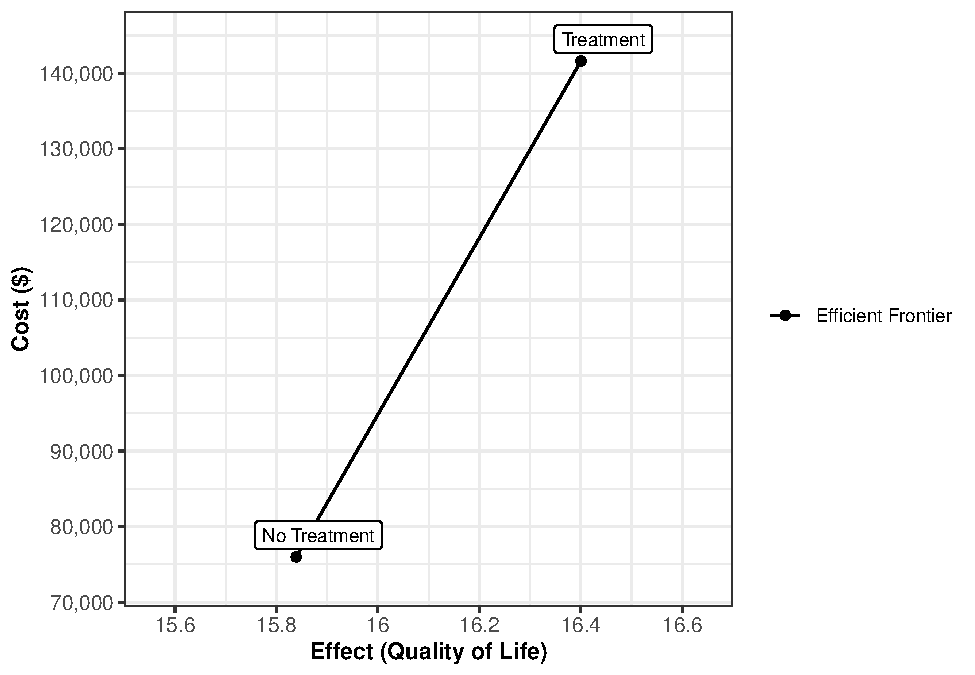
\includegraphics{decision_tree_HVE_PSA_solutions_files/figure-latex/unnamed-chunk-18-1.pdf}

\begin{Shaded}
\begin{Highlighting}[]
\CommentTok{# Initialize dataframes with PSA output }
\CommentTok{# Dataframe of costs}
\NormalTok{df_c <-}\StringTok{ }\KeywordTok{as.data.frame}\NormalTok{(}\KeywordTok{matrix}\NormalTok{(}\DecValTok{0}\NormalTok{, }
                      \DataTypeTok{nrow =}\NormalTok{ n_sim,}
                      \DataTypeTok{ncol =}\NormalTok{ n_str))}
\KeywordTok{colnames}\NormalTok{(df_c) <-}\StringTok{ }\NormalTok{v_names_str}

\CommentTok{# Dataframe of effectiveness}
\NormalTok{df_e <-}\StringTok{ }\KeywordTok{as.data.frame}\NormalTok{(}\KeywordTok{matrix}\NormalTok{(}\DecValTok{0}\NormalTok{, }
                      \DataTypeTok{nrow =}\NormalTok{ n_sim,}
                      \DataTypeTok{ncol =}\NormalTok{ n_str))}
\KeywordTok{colnames}\NormalTok{(df_e) <-}\StringTok{ }\NormalTok{v_names_str}
\end{Highlighting}
\end{Shaded}

\hypertarget{conduct-probabilistic-sensitivity-analysis}{%
\subsection{07.1 Conduct probabilistic sensitivity
analysis}\label{conduct-probabilistic-sensitivity-analysis}}

\begin{Shaded}
\begin{Highlighting}[]
\CommentTok{# Run decision tree on each parameter set of PSA input dataset}
\ControlFlowTok{for}\NormalTok{(i }\ControlFlowTok{in} \DecValTok{1}\OperatorTok{:}\NormalTok{n_sim)\{}
\NormalTok{  l_psa_input <-}\StringTok{ }\KeywordTok{update_param_list}\NormalTok{(l_params_all, df_psa_input[i, ])}
\NormalTok{  df_out_psa  <-}\StringTok{ }\KeywordTok{calculate_ce_out}\NormalTok{(l_psa_input)}
\NormalTok{  df_c[i, ] <-}\StringTok{ }\NormalTok{df_out_psa}\OperatorTok{$}\NormalTok{Cost}
\NormalTok{  df_e[i, ] <-}\StringTok{ }\NormalTok{df_out_psa}\OperatorTok{$}\NormalTok{Effect}
  \CommentTok{# Display simulation progress}
  \ControlFlowTok{if}\NormalTok{(i}\OperatorTok{/}\NormalTok{(n_sim}\OperatorTok{/}\DecValTok{10}\NormalTok{) }\OperatorTok{==}\StringTok{ }\KeywordTok{round}\NormalTok{(i}\OperatorTok{/}\NormalTok{(n_sim}\OperatorTok{/}\DecValTok{10}\NormalTok{),}\DecValTok{0}\NormalTok{)) \{ }\CommentTok{# display progress every 10%}
    \KeywordTok{cat}\NormalTok{(}\StringTok{'}\CharTok{\textbackslash{}r}\StringTok{'}\NormalTok{, }\KeywordTok{paste}\NormalTok{(i}\OperatorTok{/}\NormalTok{n_sim }\OperatorTok{*}\StringTok{ }\DecValTok{100}\NormalTok{, }\StringTok{"% done"}\NormalTok{, }\DataTypeTok{sep =} \StringTok{" "}\NormalTok{))}
\NormalTok{  \}}
\NormalTok{\}}
\end{Highlighting}
\end{Shaded}

\hypertarget{create-psa-object-for-dampack}{%
\subsection{07.2 Create PSA object for
dampack}\label{create-psa-object-for-dampack}}

\begin{Shaded}
\begin{Highlighting}[]
\NormalTok{l_psa <-}\StringTok{ }\KeywordTok{make_psa_obj}\NormalTok{(}\DataTypeTok{cost          =}\NormalTok{ df_c, }
                      \DataTypeTok{effectiveness =}\NormalTok{ df_e, }
                      \DataTypeTok{parameters    =}\NormalTok{ df_psa_input, }
                      \DataTypeTok{strategies    =}\NormalTok{ v_names_str)}
\end{Highlighting}
\end{Shaded}

\hypertarget{save-psa-objects}{%
\subsection{07.2.1 Save PSA objects}\label{save-psa-objects}}

\begin{Shaded}
\begin{Highlighting}[]
\KeywordTok{save}\NormalTok{(df_psa_input, df_c, df_e, v_names_str, n_str,}
\NormalTok{     l_psa,}
     \DataTypeTok{file =} \StringTok{"decision_tree_HVE_PSA_dataset.RData"}\NormalTok{)}
\end{Highlighting}
\end{Shaded}

\hypertarget{create-probabilistic-analysis-graphs}{%
\subsection{07.3 Create probabilistic analysis
graphs}\label{create-probabilistic-analysis-graphs}}

\begin{Shaded}
\begin{Highlighting}[]
\KeywordTok{load}\NormalTok{(}\DataTypeTok{file =} \StringTok{"decision_tree_HVE_PSA_dataset.RData"}\NormalTok{)}
\end{Highlighting}
\end{Shaded}

Vector with willingness-to-pay (WTP) thresholds.

\begin{Shaded}
\begin{Highlighting}[]
\NormalTok{v_wtp <-}\StringTok{ }\KeywordTok{seq}\NormalTok{(}\DecValTok{0}\NormalTok{, }\DecValTok{600000}\NormalTok{, }\DataTypeTok{by =} \DecValTok{10000}\NormalTok{)}
\end{Highlighting}
\end{Shaded}

\hypertarget{cost-effectiveness-scatter-plot}{%
\subsection{07.3.1 Cost-Effectiveness Scatter
plot}\label{cost-effectiveness-scatter-plot}}

\begin{Shaded}
\begin{Highlighting}[]
\KeywordTok{plot}\NormalTok{(l_psa)}
\end{Highlighting}
\end{Shaded}

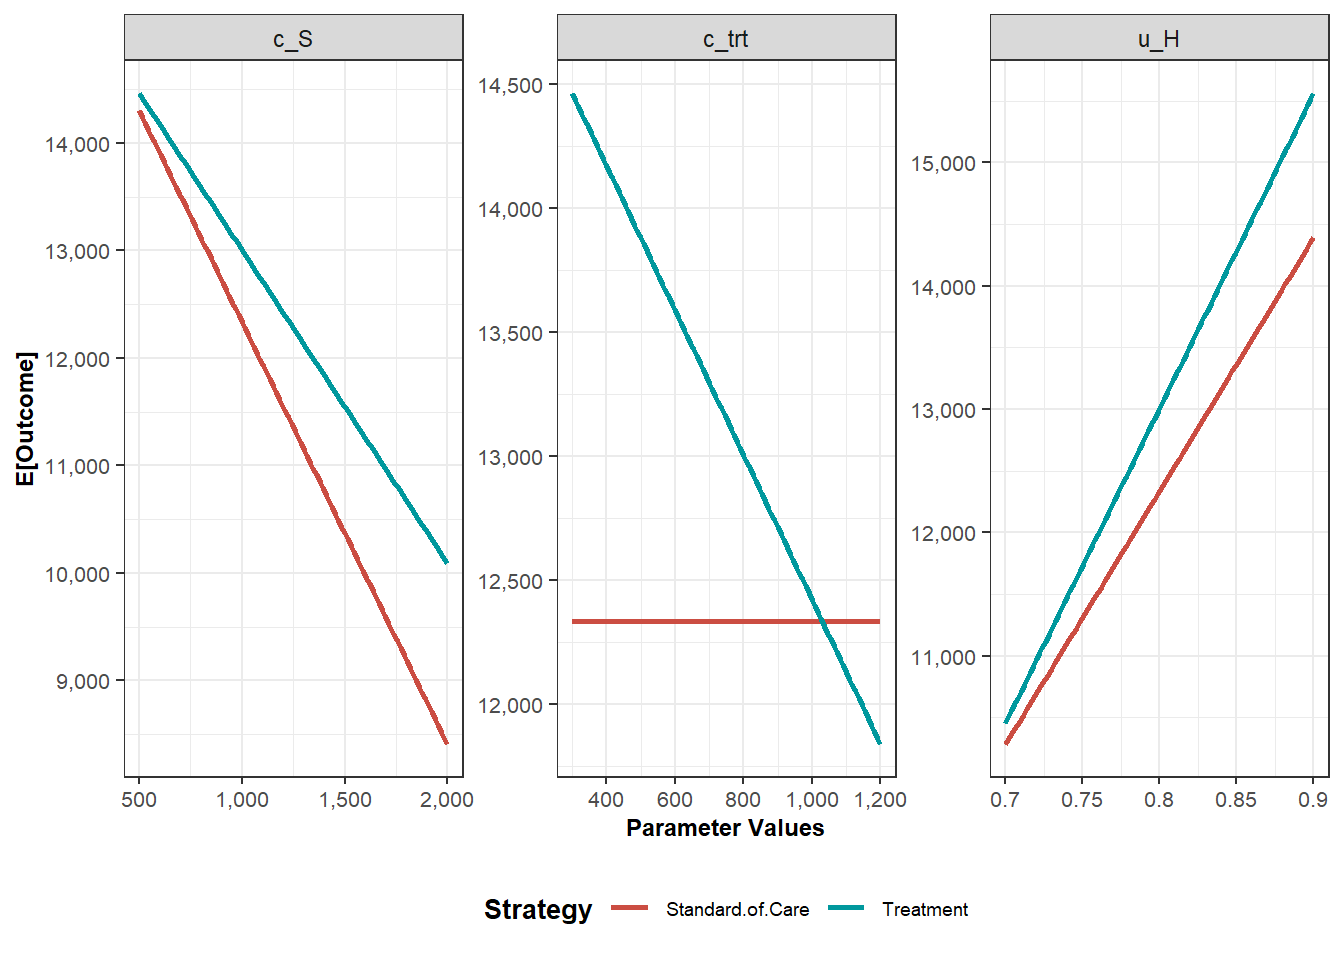
\includegraphics{decision_tree_HVE_PSA_solutions_files/figure-latex/unnamed-chunk-24-1.pdf}

\hypertarget{conduct-cea-with-probabilistic-output}{%
\subsection{07.4 Conduct CEA with probabilistic
output}\label{conduct-cea-with-probabilistic-output}}

\begin{Shaded}
\begin{Highlighting}[]
\CommentTok{# Compute expected costs and effects for each strategy from the PSA}
\NormalTok{df_out_ce_psa <-}\StringTok{ }\KeywordTok{summary}\NormalTok{(l_psa)}
\NormalTok{df_out_ce_psa}
\end{Highlighting}
\end{Shaded}

\begin{verbatim}
##   Strategy  meanCost meanEffect
## 1    No.Tx  4141.093   19.64486
## 2   Tx.All 13018.905   19.74369
## 3   Biopsy 32842.806   19.78128
\end{verbatim}

\begin{Shaded}
\begin{Highlighting}[]
\CommentTok{# Calculate incremental cost-effectiveness ratios (ICERs)}
\NormalTok{df_cea_psa <-}\StringTok{ }\KeywordTok{calculate_icers}\NormalTok{(}\DataTypeTok{cost       =}\NormalTok{ df_out_ce_psa}\OperatorTok{$}\NormalTok{meanCost, }
                              \DataTypeTok{effect     =}\NormalTok{ df_out_ce_psa}\OperatorTok{$}\NormalTok{meanEffect,}
                              \DataTypeTok{strategies =}\NormalTok{ df_out_ce_psa}\OperatorTok{$}\NormalTok{Strategy)}
\NormalTok{df_cea_psa}
\end{Highlighting}
\end{Shaded}

\begin{verbatim}
##   Strategy      Cost   Effect  Inc_Cost Inc_Effect      ICER Status
## 1    No.Tx  4141.093 19.64486        NA         NA        NA     ND
## 2   Tx.All 13018.905 19.74369  8877.813 0.09883105  89828.17     ND
## 3   Biopsy 32842.806 19.78128 19823.901 0.03758512 527440.16     ND
\end{verbatim}

\begin{Shaded}
\begin{Highlighting}[]
\CommentTok{# Save CEA table with ICERs}
\CommentTok{# As .RData}
\KeywordTok{save}\NormalTok{(df_cea_psa, }
     \DataTypeTok{file =} \StringTok{"decision_tree_HVE_probabilistic_CEA_results.RData"}\NormalTok{)}
\CommentTok{# As .csv}
\KeywordTok{write.csv}\NormalTok{(df_cea_psa, }
          \DataTypeTok{file =} \StringTok{"decision_tree_HVE_probabilistic_CEA_results.csv"}\NormalTok{)}
\end{Highlighting}
\end{Shaded}

\hypertarget{plot-cost-effectiveness-frontier}{%
\subsection{07.4.1 Plot cost-effectiveness
frontier}\label{plot-cost-effectiveness-frontier}}

\begin{Shaded}
\begin{Highlighting}[]
\KeywordTok{plot}\NormalTok{(df_cea_psa) }
\end{Highlighting}
\end{Shaded}

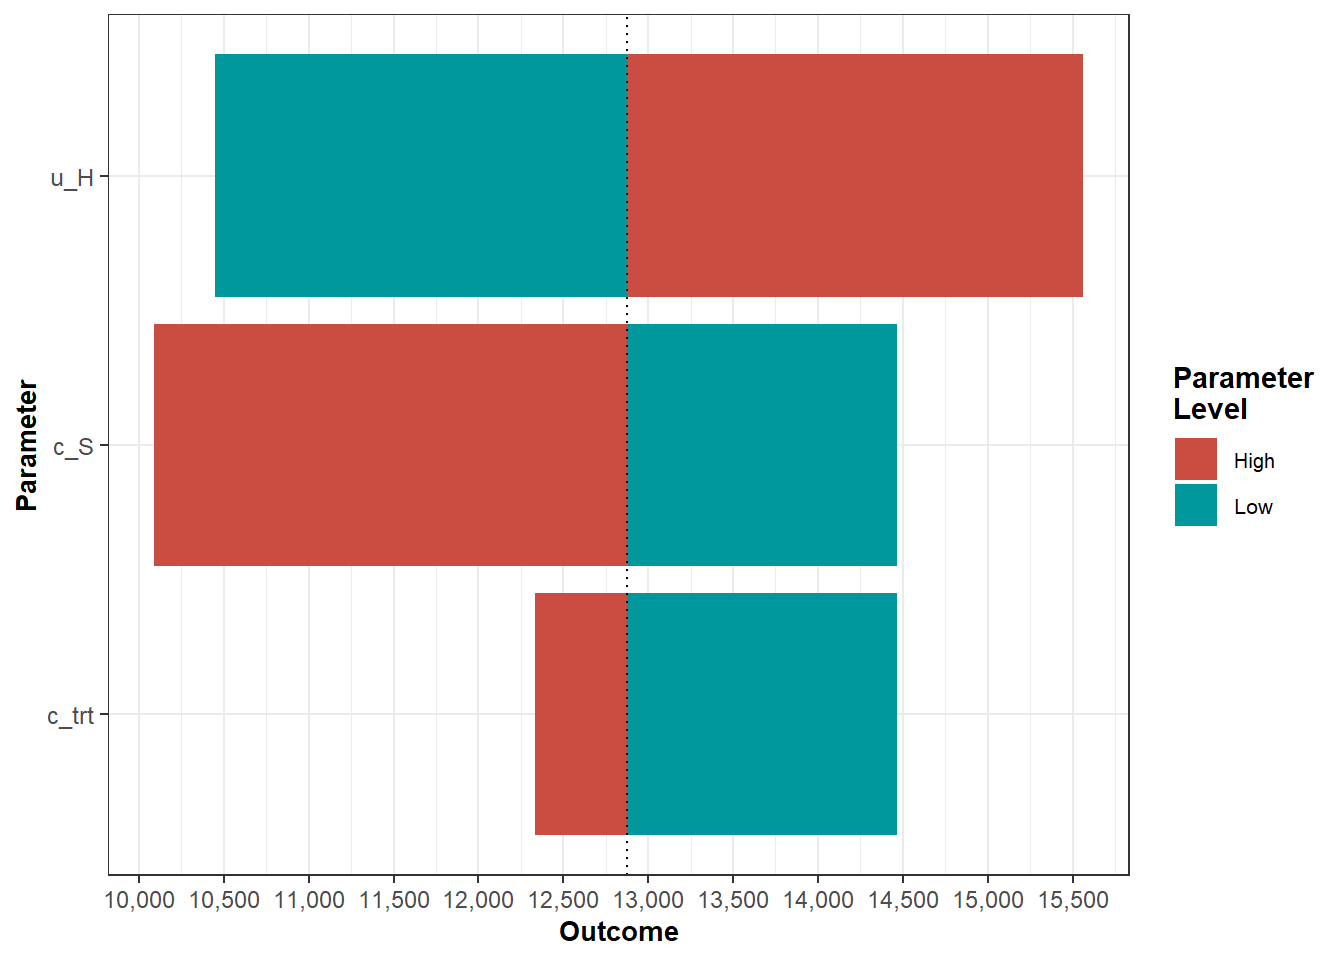
\includegraphics{decision_tree_HVE_PSA_solutions_files/figure-latex/unnamed-chunk-26-1.pdf}

\hypertarget{cost-effectiveness-acceptability-curves-ceacs-and-frontier-ceaf}{%
\subsection{07.4.2 Cost-effectiveness acceptability curves (CEACs) and
frontier
(CEAF)}\label{cost-effectiveness-acceptability-curves-ceacs-and-frontier-ceaf}}

\begin{Shaded}
\begin{Highlighting}[]
\NormalTok{ceac_obj <-}\StringTok{ }\KeywordTok{ceac}\NormalTok{(}\DataTypeTok{wtp =}\NormalTok{ v_wtp, }\DataTypeTok{psa =}\NormalTok{ l_psa)}
\CommentTok{# Regions of highest probability of cost-effectiveness for each strategy}
\KeywordTok{summary}\NormalTok{(ceac_obj)}
\end{Highlighting}
\end{Shaded}

\begin{verbatim}
##   range_min range_max cost_eff_strat
## 1         0     90000          No.Tx
## 2         0    530000         Tx.All
## 3     90000    600000         Tx.All
## 4    530000    600000         Biopsy
## 5    530000        NA         Biopsy
\end{verbatim}

\begin{Shaded}
\begin{Highlighting}[]
\CommentTok{# CEAC & CEAF plot}
\KeywordTok{plot}\NormalTok{(ceac_obj)}
\end{Highlighting}
\end{Shaded}

\includegraphics{decision_tree_HVE_PSA_solutions_files/figure-latex/unnamed-chunk-27-1.pdf}

\hypertarget{expected-loss-curves-elcs}{%
\subsection{07.4.3 Expected Loss Curves
(ELCs)}\label{expected-loss-curves-elcs}}

\begin{Shaded}
\begin{Highlighting}[]
\NormalTok{elc_obj <-}\StringTok{ }\KeywordTok{calc_exp_loss}\NormalTok{(}\DataTypeTok{wtp =}\NormalTok{ v_wtp, }\DataTypeTok{psa =}\NormalTok{ l_psa)}

\CommentTok{# ELC plot}
\KeywordTok{plot}\NormalTok{(elc_obj, }\DataTypeTok{log_y =} \OtherTok{FALSE}\NormalTok{)}
\end{Highlighting}
\end{Shaded}

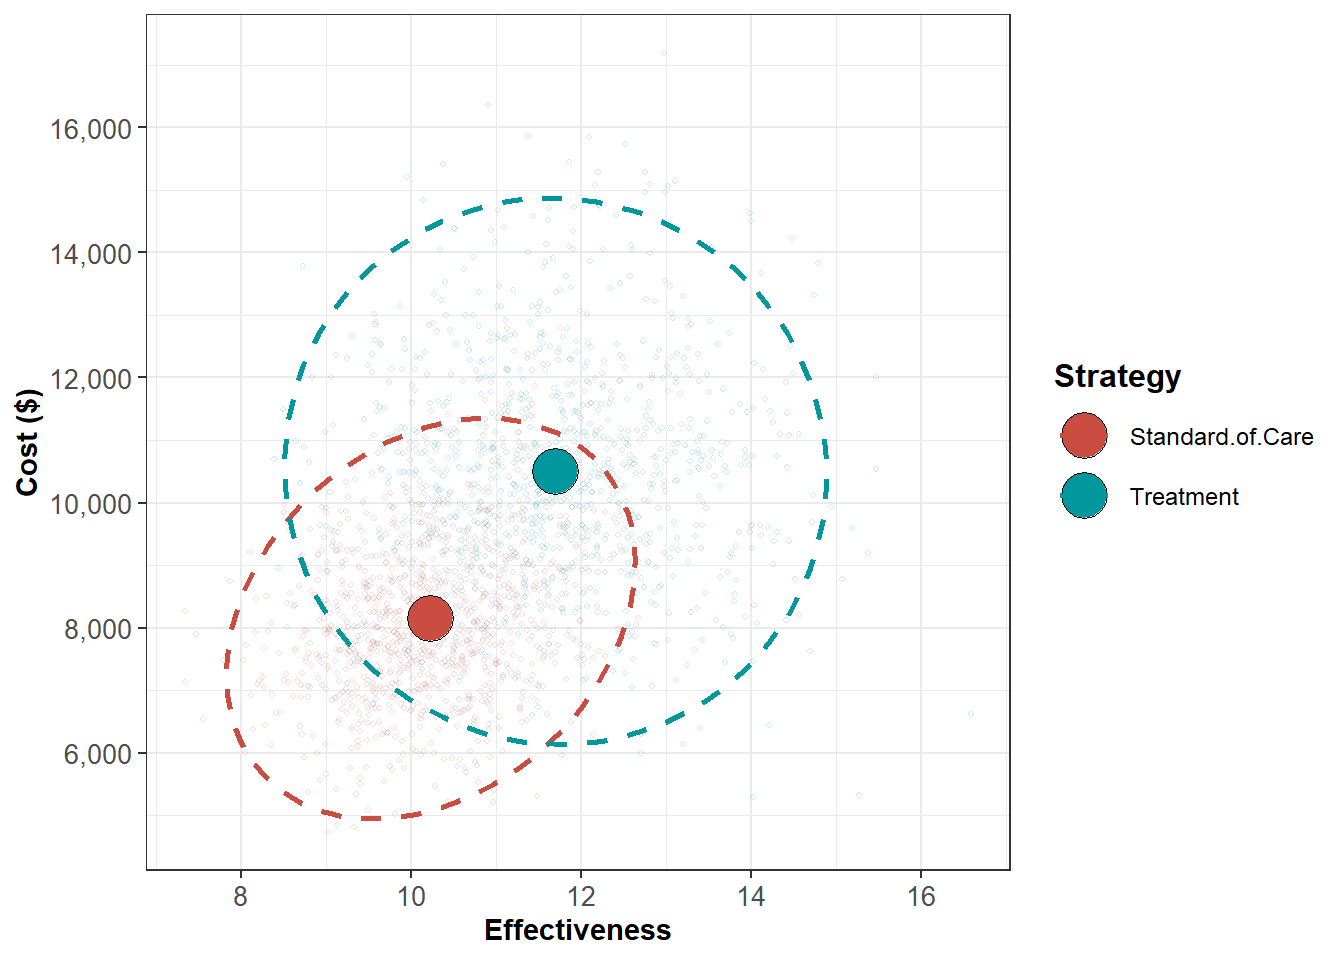
\includegraphics{decision_tree_HVE_PSA_solutions_files/figure-latex/unnamed-chunk-28-1.pdf}

\hypertarget{expected-value-of-perfect-information-evpi}{%
\subsection{07.4.4 Expected value of perfect information
(EVPI)}\label{expected-value-of-perfect-information-evpi}}

\begin{Shaded}
\begin{Highlighting}[]
\NormalTok{evpi <-}\StringTok{ }\KeywordTok{calc_evpi}\NormalTok{(}\DataTypeTok{wtp =}\NormalTok{ v_wtp, }\DataTypeTok{psa =}\NormalTok{ l_psa)}
\CommentTok{# EVPI plot}
\KeywordTok{plot}\NormalTok{(evpi, }\DataTypeTok{effect_units =} \StringTok{"QALY"}\NormalTok{) }
\end{Highlighting}
\end{Shaded}

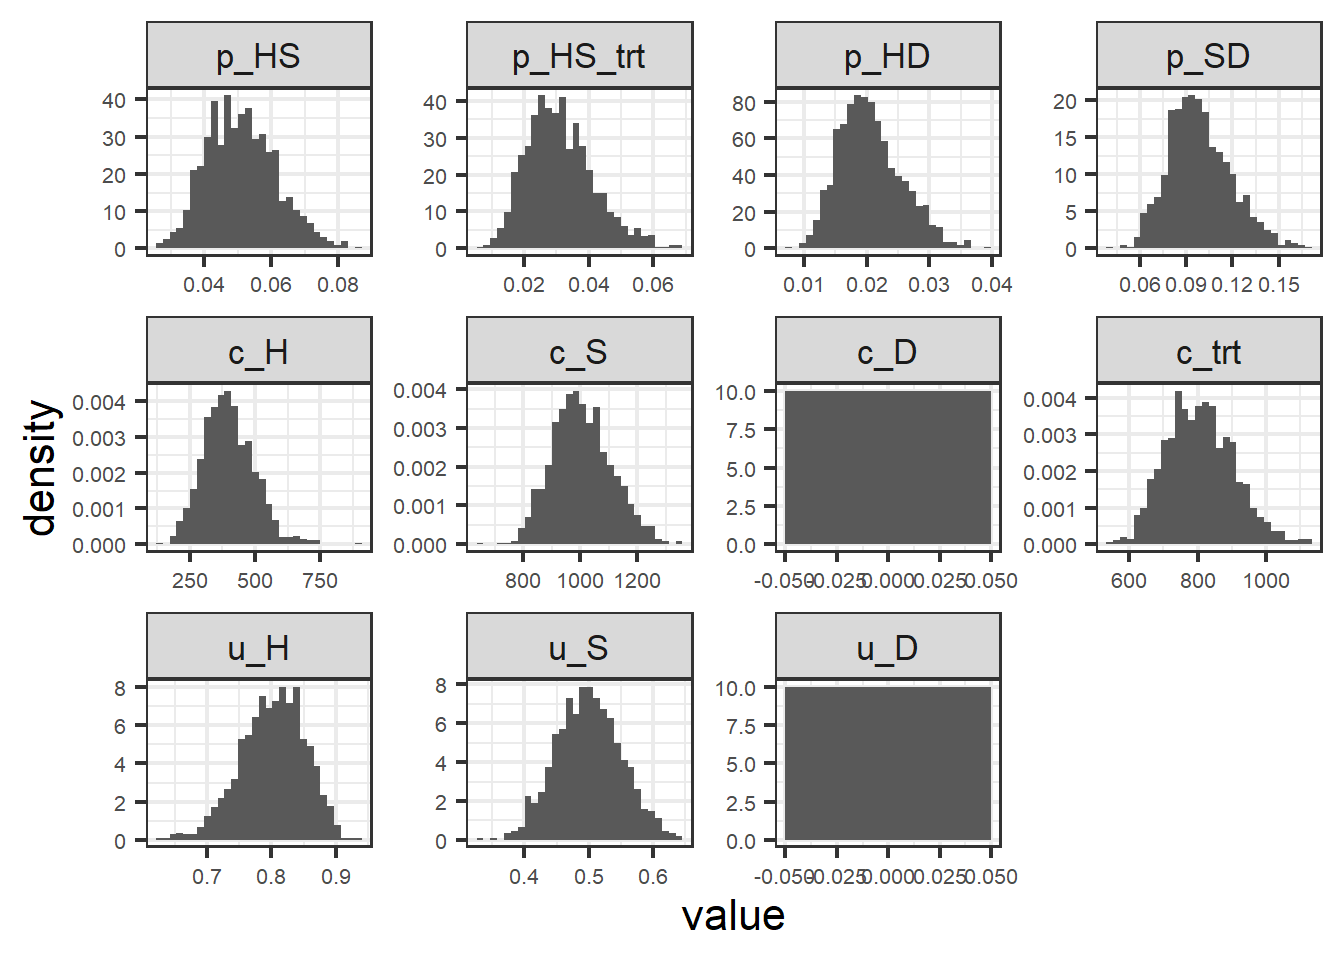
\includegraphics{decision_tree_HVE_PSA_solutions_files/figure-latex/unnamed-chunk-29-1.pdf}

\hypertarget{expected-value-of-partial-perfect-information-evppi}{%
\subsection{07.4.5 Expected value of partial perfect information
(EVPPI)}\label{expected-value-of-partial-perfect-information-evppi}}

\begin{Shaded}
\begin{Highlighting}[]
\NormalTok{evppi <-}\StringTok{ }\KeywordTok{calc_evppi}\NormalTok{(}\DataTypeTok{psa =}\NormalTok{ l_psa, }
                    \DataTypeTok{wtp =}\NormalTok{ v_wtp, }
                    \DataTypeTok{params =} \KeywordTok{c}\NormalTok{(}\StringTok{"q_VE_comp"}\NormalTok{), }
                    \DataTypeTok{outcome =} \KeywordTok{c}\NormalTok{(}\StringTok{"nmb"}\NormalTok{),}
                    \DataTypeTok{type =} \KeywordTok{c}\NormalTok{(}\StringTok{"gam"}\NormalTok{, }\StringTok{"poly"}\NormalTok{),}
                    \DataTypeTok{poly.order =} \DecValTok{2}\NormalTok{,}
                    \DataTypeTok{k =} \DecValTok{-1}\NormalTok{,}
                    \DataTypeTok{pop =} \DecValTok{1}
\NormalTok{)}

\NormalTok{dampack}\OperatorTok{:::}\KeywordTok{plot.evppi}\NormalTok{(evppi)}
\end{Highlighting}
\end{Shaded}

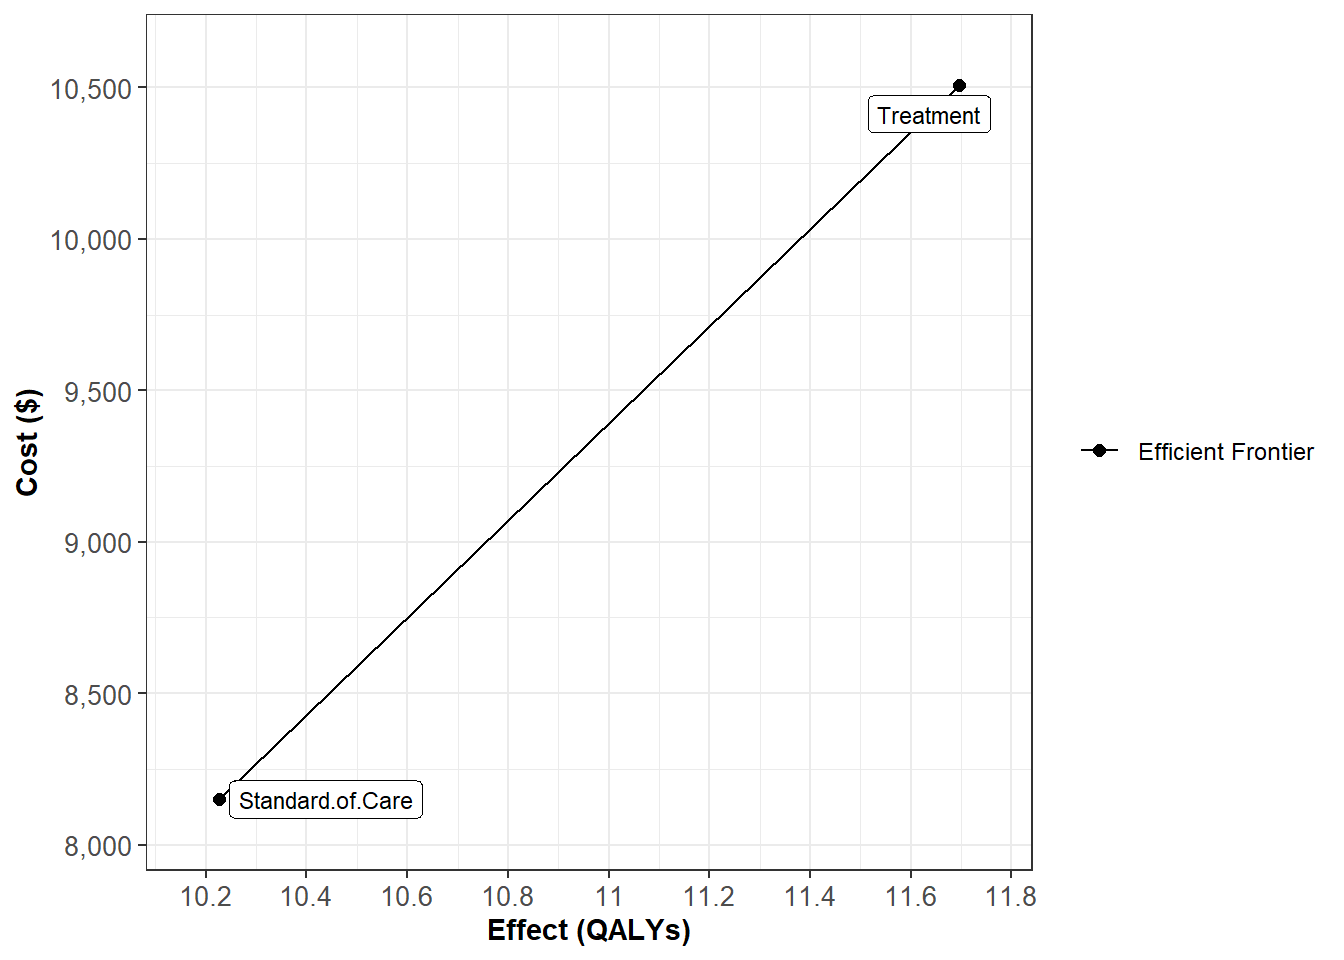
\includegraphics{decision_tree_HVE_PSA_solutions_files/figure-latex/unnamed-chunk-30-1.pdf}

\end{document}
